\chapter{Einleitung}
\begin{multicols}{2}
\raggedcolumns
\noindent Die vorliegende Arbeit widmet sich der Auswertung von Funden und Befunden, die in den 1980er Jahren im nordwestlichen Teil des Kongobeckens gemacht wurden. Sie verfolgt dabei das Ziel, Charakter und Verlauf der Besiedlung der Region durch keramikproduzierende, sesshaftlebende und nahrungsmittelanbauende Bevölkerungen nachzuzeichnen. Die in dieser Arbeit diskutierten Materialien stammen aus den Prospektions- und Grabungsaktivitäten des unter der Leitung von Manfred K.~H.~Eggert durchgeführten \textit{River Reconnaissance Project}. Der durch das Projekt erstmals archäologisch erschlossene Untersuchungsraum \parencite[siehe][295 Abb.~16.2]{Eggert.1993} kann in zwei Teile untergliedert werden: zum einen das sogenannte \enquote*{Innere Kongobecken}, welches durch die Prospektionen der linksseitigen Zuflüsse des Kongoflusses repräsentiert wird und Gegenstand einer bis in die Anfänge der 1990er Jahre andauernden Auswertungs- und Publikationstätigkeit war \parencites{Eggert.1980b}{Eggert.1981}{Eggert.1983}{Eggert.1984}{Eggert.1984b}{Eggert.1987}{Wotzka.1995}, sowie das Arbeitsgebiet der vorliegenden Arbeit, das \enquote*{nordwestliche Kongobecken}.\footnote{In Methodik (siehe Kap.~\ref{sec:Quellen}) wie der Beschreibung der keramischen Inventare (siehe Kap.~\ref{sec:Keramiksequenz}, \ref{sec:Horizonte}) orientiert sich die vorliegende Arbeit an der Vorlage der archäologisch erschlossenen Keramiksequenz für das Innere Kongobecken durch Hans-Peter \textsc{Wotzka} (1995).} Dieses, die rechtsseitigen Zuflüsse des Kongo umfassende Gebiet und sein archäologisches Potenzial waren bislang lediglich Gegenstand einiger Vorberichte \parencites{Eggert.1987c}{Eggert.1992}{Eggert.1993}. 

Zur Erarbeitung des räumlich-zeitlichen Bezugssystems wurde die aus dem Arbeitsgebiet vorliegende Gefäßkeramik herangezogen. Neben der Tatsache, dass es sich bei der Gefäßkeramik um die umfangreichste Fundkategorie handelt (Tab.~\ref{tab:Funde_Uebersicht}), eignet sie sich für einen strukturellen Vergleich vor allem aufgrund ihrer potenziellen Präsenz im Alltag der zu untersuchenden Gesellschaften.\footnote{Die zentrale Rolle der Gefäßkeramik bei der Beurteilung prähistorischer Sachkultur wurde zuletzt intensiv von \textcite{Saev.2015} beleuchtet. Gegenstand dieser Untersuchung war die Funktion und Nutzung von Gefäßkeramik im südlichen Ostseeraum vom Neolithikum bis zur Zeitenwende. Ebenfalls sei für die Fragestellung nach der Nutzung und Funktion von prähistorischer Gefäßkeramik auf die Diskussion zwischen \textcites{Riemer.1997}{Wotzka.1997}{Veit.1997} sowie den ethnoarchäologisch ausgerichteten Beitrag von \textcite{Knopf.2009} verwiesen.} Der in dieser Arbeit gewählte Fokus auf die Gefäßkeramik des Arbeitsgebietes setzt eine kontinuierliche Nutzung von Keramik von ihrem ersten archäologisch nachgewiesenen Auftreten bis in die Gegenwart (1985/87) voraus. Diese Annahme bildet in der Folge die Voraussetzung für den diachronen Vergleich (Kap.~\ref{sec:BesiedlGesch}). Ausgangspunkt bildeten dabei die Inventare von insgesamt 19 ausgegrabenen oder hinreichend archäologisch untersuchten Befunden (Katalog~A). Sie wurden um Inventare ergänzt, die bei Surveys innerhalb der modernen Dörfer erschlossen wurden (Katalog B). Die Untersuchung der Quellen vollzieht sich auf zwei Ebenen: Auf die Auseinandersetzung mit Indizien zur Keramiktechnologie (Kap.~\ref{sec:Herstellung}) folgt eine detaillierte Beschreibung von vornehmlich auf stilistischem Wege erarbeiteten keramischen Gruppen, im Weiteren \enquote*{Stilgruppen} genannt (Kap.~\ref{sec:Keramiksequenz}). Sie bilden die grundlegende Entität für die Rekonstruktion der Besiedlungsgeschichte des Arbeitsgebietes (Kap.~\ref{sec:BesiedlGesch}).

Rückschlüsse auf den Charakter sowie Verlauf der Besiedlung des Kongobeckens durch keramikproduzierende, sesshaftlebende und nahrungsmittelanbauende Gruppen lassen sich zum gegenwärtigen Zeitpunkt lediglich auf Grundlage einer sehr eingeschränkten Quellenbasis ziehen. Ausschließlich im Rahmen des \textit{River Reconnaissance Project} wurden bisher systematisch Prospektionen sowie Grabungen durchgeführt. Regionale Abfolgen des keramischen Fundmaterials\footnote{Im weiteren Text wird für die Abfolge der keramischen Stile (siehe auch Kap.~\ref{sec:Sequenzen}) der Begriff \enquote{Sequenz} genutzt.} und daraus ableitbare chronologische Gliederungen liegen lediglich für ausgewählte Regionen vor \parencites{Wotzka.1995}{MbidaMindzie.19951996}{AssokoNdong.20002001}{Clist.20042005}{Lavachery.2010}. Weite Teile Zentralafrikas\footnote{Unter \enquote*{Zentralafrika} wird im Sinne dieser Arbeit das Staatsgebiet Äquatorialguineas, Gabuns, Kameruns, der Demokratischen Republik Kongo (Kongo-Kinshasa), der Republik Kongo (Kongo-Brazzaville) und der Zentralafrikanischen Republik sowie der nördliche Teil Angolas verstanden \parencite[183]{Eggert.2014}. Verschiedentlich werden auch noch der Süden des Tschads sowie Ruanda und Burundi zu diesem Raum hinzu gezählt \parencite[421]{Maret.2005}.} sind bis heute archäologische \textit{terra incognita}.

\section{Arbeitsgebiet und Fragestellung}\label{sec:Arbeitsgebiet}

Unter der Bezeichnung \enquote*{nordwestliches Kongobecken} werden in dieser Arbeit die 1985 und 1987 durch das \textit{River Reconnaissance Project} befahrenen Flussabschnitte des \mbox{Sangha}, \mbox{Ngoko}, Likwala-aux-Herbes, \mbox{Ubangi} und Lua sowie ein kurzes verbindendes Stück entlang des Kongo zwischen der \mbox{Ubangi}- und \mbox{Sangha}-Mündung verstanden (Abb.~\ref{fig:ArbeitsgebietKarte}). Das eigentliche Arbeitsgebiet umfasst administrativ vor allem den nordöstlichen Teil der Republik Kongo (Kongo-Brazzaville) sowie unmittelbar angrenzende Regionen Kameruns, der Zentralafrikanischen Republik und der Demokratischen Republik Kongo (Kongo-Kinshasa). Im nördlichen Teil, entlang des oberen \mbox{Ubangi}, deckt das Arbeitsgebiet die Grenzen der heutigen Provinzen Süd-\mbox{Ubangi} sowie Nord-\mbox{Ubangi} ab.

\begin{figure*}[p]
	\centering
	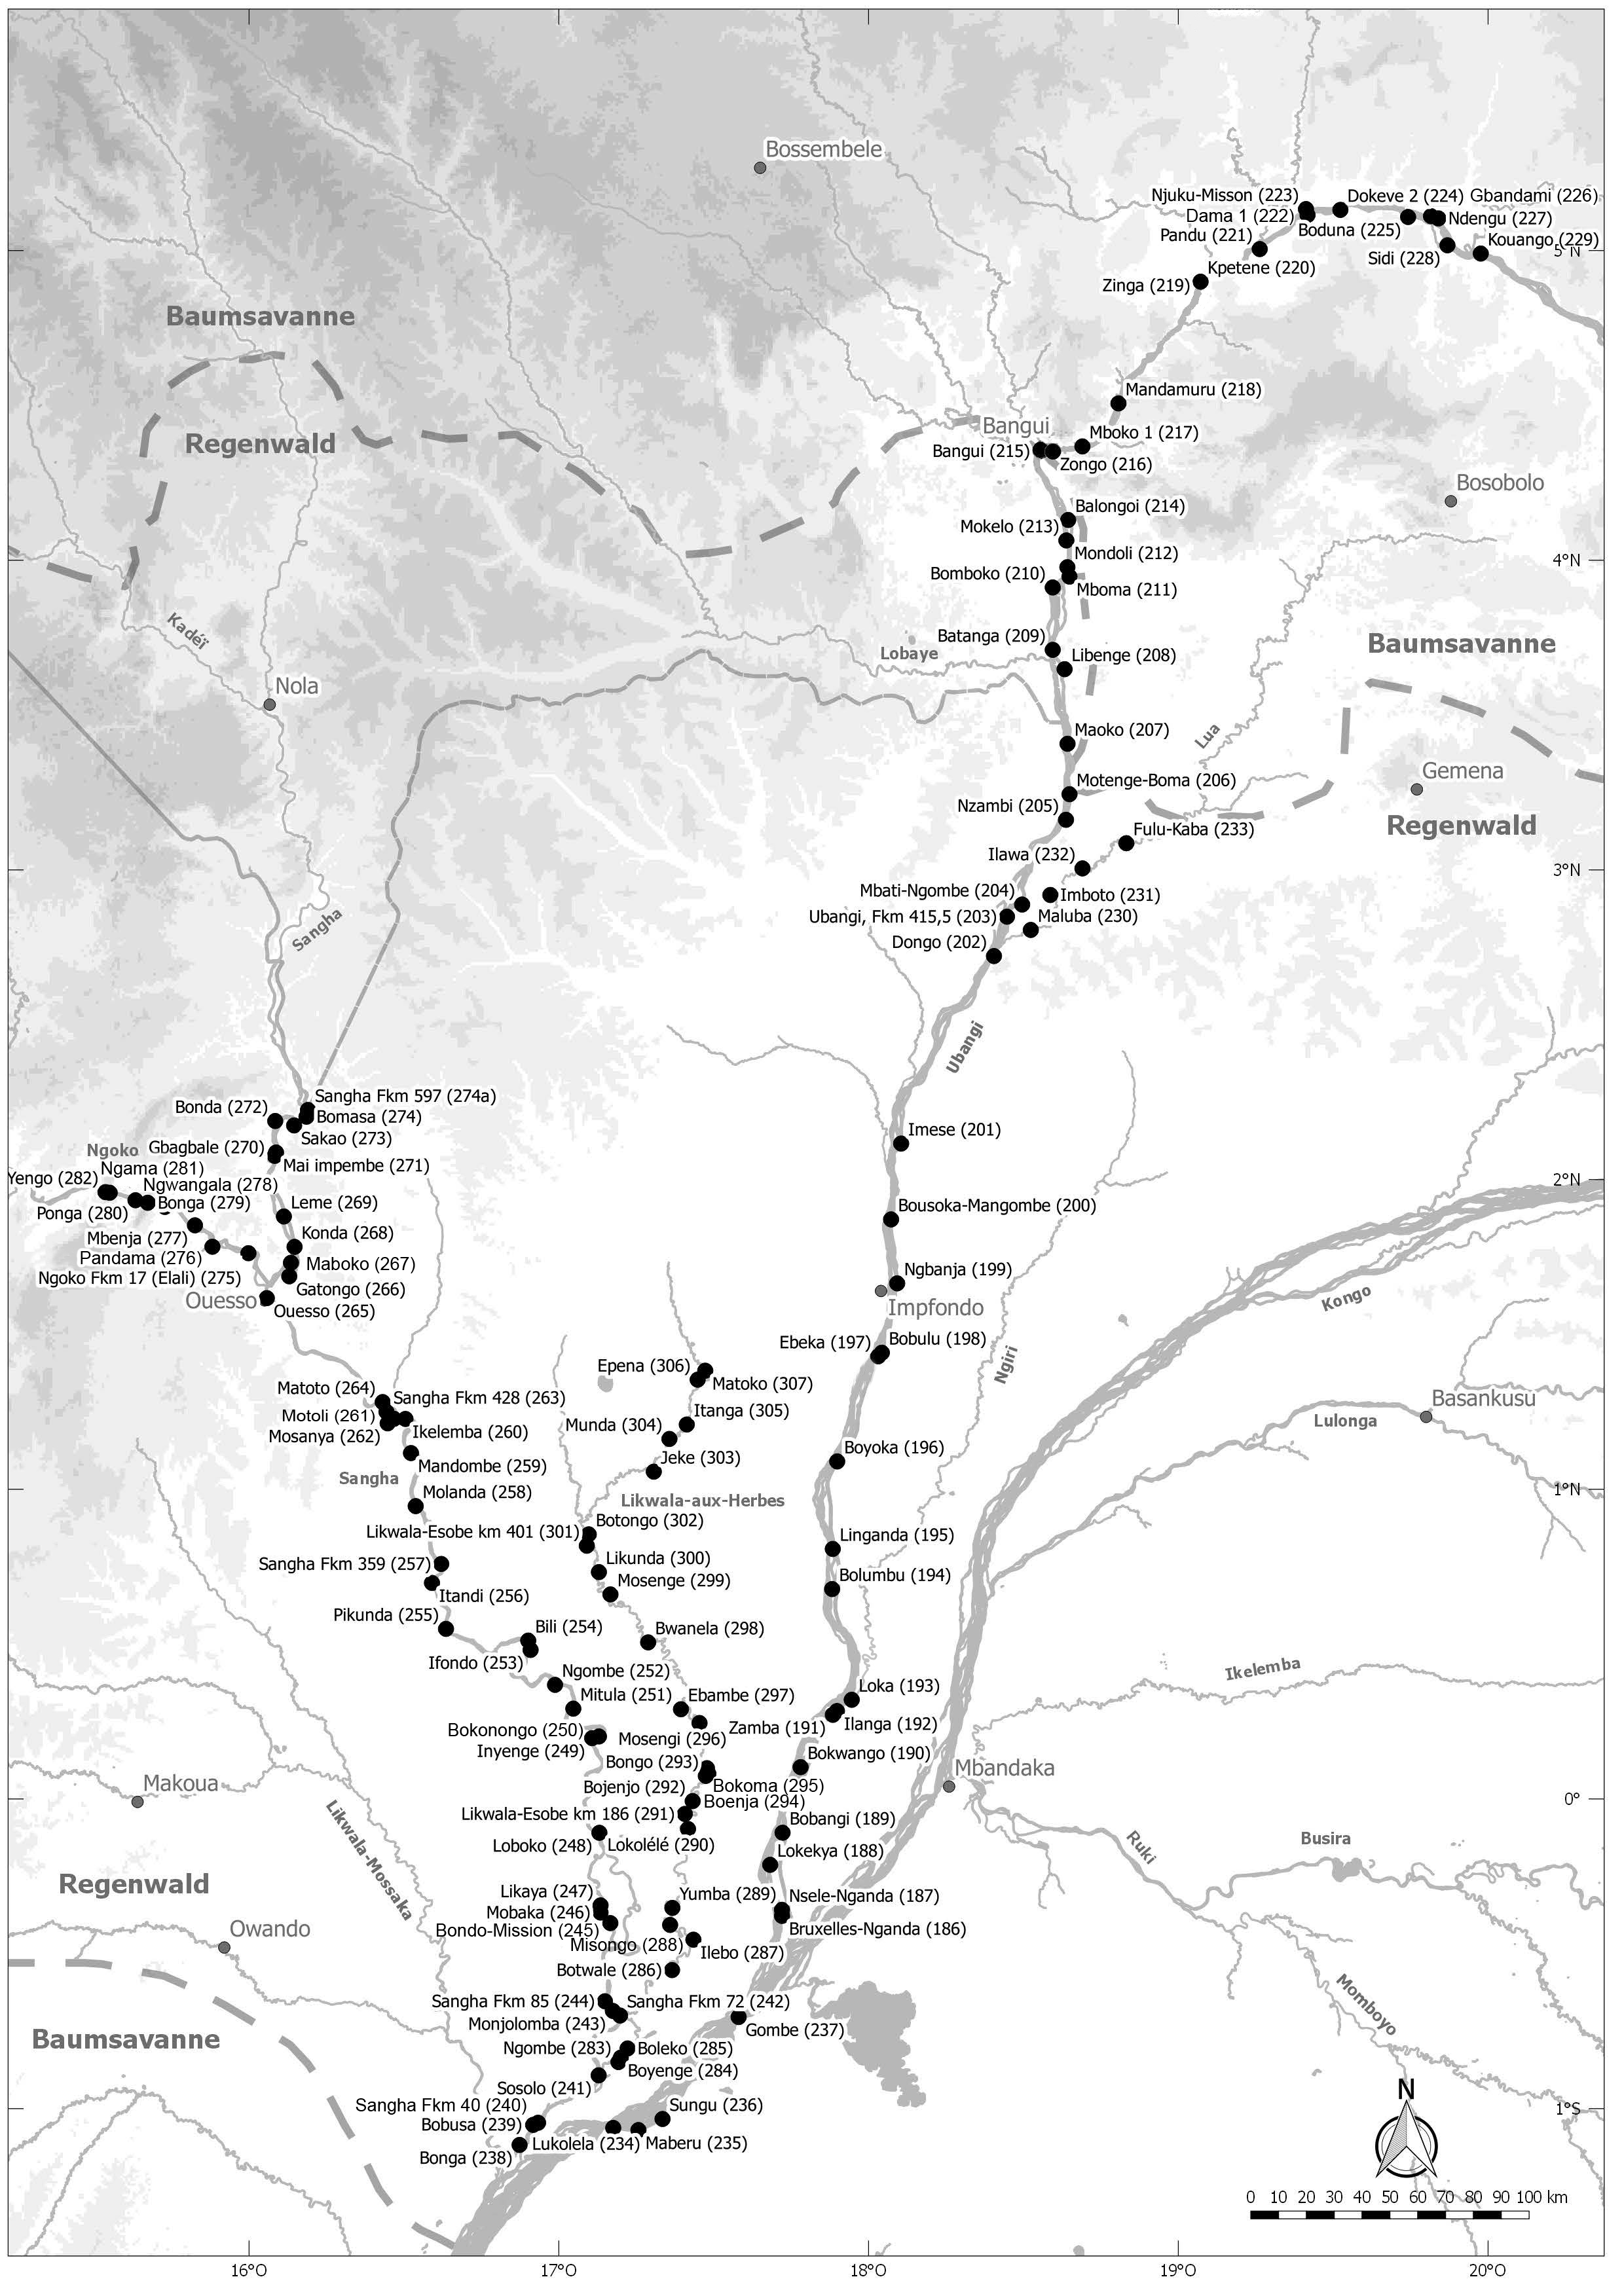
\includegraphics[width=\textwidth]{fig/FundstellenMap.jpg}
	\caption{Arbeitsgebiet: Untersuchte Fundstellen}
	\label{fig:ArbeitsgebietKarte}
\end{figure*}

Das Arbeitsgebiet beschreibt einen Nord--Süd-Transekt von der Feuchtsavanne nördlich von Bangui (Zentralafrikanische Republik) bis in den äquatorialen Regenwald südlich von Mba\-ndaka (Demokratische Republik Kongo). In Nord--Süd-Richtung erstreckt es sich über 700\,km, während es in Ost--West-Richtung annähernd 500\,km groß ist. Alle Fundstellen liegen zwischen 289--390\,m\,ü.\,NN.\footnote{Die Höhen der Fundstellen wurden einem SRTMv3-Datensatz mit einer Grundauflösung von 3 Bogensekunden beziehungsweise etwa 90\,m entnommen (Quelle NASA/USGS; \url{https://earthexplorer.usgs.gov} Zugriff: 04.\,10.\,2014).}

Die Feldarbeiten des \textit{River Reconnaissance Project} in der zweiten Hälfte der Kampagne von 1985 sowie während der Kampagne von 1987 deckten etwa 2130\,km der Flussläufe des \mbox{Ubangi}, Lua, \mbox{Sangha}, \mbox{Ngoko} und \mbox{Likwala}-\mbox{aux}-\mbox{Herbes} ab (Tab.~\ref{tab:ArbeitsgebietFlussstrecken}). Ausgehend von seiner Mündung in den \mbox{Sangha}, die etwa 3\,km nördlich von Ouesso (Fpl.~265) liegt, wurde der \mbox{Ngoko} auf einer Strecke von etwa 80\,km stromauf prospektiert.\footnote{Der untere Abschnitt des Dja, der in Kamerun entspringt, wird ab dem Punkt, an dem er die Grenze zwischen Kamerun und der Republik Kongo bildet (2$^\circ$12$'$25$''$~N, 14$^\circ$35$'$42$''$~O) als \enquote*{\mbox{Ngoko}} bezeichnet. In Yengo (Fpl.~282) musste die Prospektion aufgrund der Malaria-Erkrankung eines Mitarbeiters vorzeitig beendet werden.\label{ftn:DjaNgoko}} Der \mbox{Sangha} bildet den Unterlauf des Kadeï, der in Nordkamerun nahe Garoua-Bouleï entspringt und ab Nola (Zentralafrikanische Republik) als \mbox{Sangha} bezeichnet wird. Der Fluss mündet bei Mossaka, etwa 220\,km südwestlich von Mbandaka in den Kongo. Er wurde auf einer Länge von fast 600\,km bis an das Dreiländereck der Republik Kongo, Kamerun und der Zentralafrikanischen Republik knapp nördlich von Bomasa (Fpl.~274) befahren. Zwischen den Flüssen \mbox{Sangha} und \mbox{Ubangi} liegt der Likwala-aux-Herbes, der auch als \enquote*{Likwala-Esobe} oder \enquote*{Likouala-aux-Herbes} bezeichnet wird und nordwestlich des Lac Tele entspringt. Der \mbox{Likwala}-\mbox{aux}-\mbox{Herbes} wurde insgesamt auf einer Strecke von über 500\,km prospektiert, bis zur nicht passierbaren Brücke bei Matoko (Fpl.~307).\footnote{Der Fluss darf nicht mit dem Likwala-Mossaka verwechselt werden, der auf einigen Karten nur mit der Bezeichnung \enquote*{Likwala} verzeichnet ist. Er verläuft westlich des \mbox{Sangha} und mündet bei Mossaka, wie auch der \mbox{Sangha}, in den Kongo.} Der \mbox{Ubangi} zählt zu den größten Zuflüssen des Kongo und bildet die Grenze zwischen der Demokratischen Republik Kongo und der Zentralafrikanischen Republik sowie der Republik Kongo. Er entspringt aus dem Zusammenfluss von Uele und Mbomou bei Yakoma (Demokratische Republik Kongo) und mündet etwa 90\,km südwestlich von Mbandaka in den Kongo. Der \mbox{Ubangi} wurde auf einer Strecke von etwa 850\,km, bis Kouango (Fpl.~229) befahren. Der Lua ist neben dem Ngiri einer der größten linksseitigen Zuflüsse des \mbox{Ubangi}. Er mündet bei Dongo (Fpl.~202) in den \mbox{Ubangi} und wurde auf einer Strecke von etwa 100\,km bis Fulu-Kaba (Fpl.~233) prospektiert.

\vspace{1.5em}
\noindent Durch diese Feldarbeiten der 1980er Jahre ließen sich für die in dieser Arbeit präsentierte Erstbearbeitung der Befunde und Funde aus dem nordwestlichen Kongobecken eine Reihe von Fragestellungen und Arbeitsziele formulieren:
\begin{itemize*}
\item Die Auswertung der ausgegrabenen Befunde in Maluba (Fpl.~230; Kat.-Nr.~1--5), Bobusa (Fpl.~239; Kat.-Nr.~6--7), Pikunda (Fpl.~255; Kat.-Nr.~8--10), Boleko (Fpl.~285; Kat.-Nr.~14) und Munda (Fpl.~304; Kat.-Nr.~15--18).
\item Die Aufnahme und Auswertung der noch nicht bearbeiten Keramik des \textit{River Reconnaissance Project} aus den Feldkampagnen von 1985 (Flüsse: \mbox{Ubangi} und Lua) und 1987 (Flüsse: \mbox{Sangha}, \mbox{Ngoko} und Likwala-aux-Herbes).
\item Die Formulierung einer Besiedlungsabfolge für die befahrenen Flussläufe des \mbox{Sangha}/\mbox{Ngoko}, \mbox{Likwala}-\mbox{aux}-\mbox{Herbes} und \mbox{Ubangi}/Lua.
\item Ein Vergleich der erarbeiteten archäologischen Sequenz mit benachbarten Regionen, allen voran dem von \textcite{Wotzka.1995} untersuchten Inneren Kongobecken.
\end{itemize*}
\vfill
\noindent\begin{minipage}[b]{\columnwidth}
	{\footnotesize \begin{sftabular}{@{}p{.2\textwidth}R{.2\textwidth}p{.49\textwidth}@{}}
			\toprule
			\textbf{Flusslauf} & \textbf{Befahrung} & \textbf{Endpunkt} \\
			\midrule
			\mbox{Ubangi} & 850\,km & Kouango (Fpl.~229) \\
			Lua & 97\,km & Fulu-Kaba (Fpl.~233) \\
			Kongo/Za{\"i}re & 60\,km & Zwischen Gombe (Fpl.~234) und Lokolela (Fpl.~237) \\
			\mbox{Sangha} & 597\,km & Bomasa (Fpl.~274a) \\
			\mbox{Ngoko} & ca. 80\,km & Yengo (Fpl.~282)\\
			Likwala-aux-Herbes & 526\,km & Matoko (Fpl.~307) \\
			\bottomrule
	\end{sftabular}}
	\captionof{table}{Arbeitsgebiet: Prospektierte Flussabschnitte (siehe Abb.~\ref{fig:ArbeitsgebietKarte})\label{tab:ArbeitsgebietFlussstrecken} \vspace{2.75em}}
\end{minipage}
\noindent Aus diesen Hauptzielen ergaben sich eine Reihe von Kernfragen:
\begin{itemize*}
\item Welche keramischen Stilgruppen lassen sich vor dem Hintergrund der beobachtbaren Variabilität keramischer Formen im Arbeitsgebiet formulieren?
\item Welche Rückschlüsse lassen sich von Eigenschaften sowie Spuren an der Gefäßkeramik auf die Herstellungstechniken herleiten?
\item Welches sind die ältesten im Arbeitsgebiet anzutreffenden keramischen Stilgruppen?
\item Welche relativ- sowie absolutchronologischen Verbindungen bestehen zwischen den einzelnen keramischen Stilgruppen des Arbeitsgebietes?
\item Welche Beziehungen bestehen zwischen den keramischen Stilgruppen des nordwestlichen Kongobeckens und denen der umgebenden Regionen, vor allem dem Inneren Kongobecken?
\item Welche keramischen Stilgruppen des Inneren Kongobeckens können auch im nordwestlichen Kongobecken beobachtet werden?
\item Welche Konsequenzen ergeben sich aus den neu hinzugewonnenen Erkenntnissen aus der Sequenz des nordwestlichen Kongobeckens für die Besiedlungsgeschichte des Kongobeckens allgemein?
\end{itemize*}

\section{Forschungsgeschichte}

\paragraph{Feldforschung vor 1977}\hspace{-.5em}|\hspace{.5em}%
Die Geschichte der archäologischen Erforschung des Kongobeckens bis in die späten 1980er Jahre, mit besonderem Fokus auf das Innere Kongobecken, wurde durch \textsc{Wotzka} (ebd. 22--31) systematisch vorgestellt. Die erste archäologische Ausgrabung im nordwestlich angrenzenden Arbeitsgebiet wurde 1968 durch Roger \textcite{deBayledesHermens.1975} in Batalimo am linken Ufer des Lobaye (Abb.~\ref{fig:BTM-Verbreitung}), einem Zufluss des \mbox{Ubangi}, durchgeführt. Durch einen kleinen Testschnitt von 6\,m\textsuperscript{2} (2\,\( \times \)\,3\,m; ebd. 206--221) wurde in einer \enquote*{Kulturschicht} Keramik sowie Steinartefakte erfasst (\textsc{De Bayle des Hermens} 1975: Taf.~32). Bereits bei der Grabung konnten zwei keramische Gruppen unterschieden werden: flachbodige, reich verzierte Gefäße und einfache, unverzierte Töpfe mit sich leicht verengender Öffnung \parencites[224, 234]{Aumassip.1975}[134]{Eggert.1987c}. Eine dem reich verzierten Material aus Batalimo entsprechende Keramik wurde 1985 auch von \textsc{Eggert} (ebd. 137--141) an der Fundstelle Maluba am Lua (Fpl.~230) entdeckt und in Zusammenschau mit den älteren Funden vom Lobaye unter der Bezeichnug \enquote*{Batalimo-Maluba-Gruppe} subsumiert (siehe Kap.~\ref{sec:BTM-Gr}).

Zwischen Dezember 1972 und März 1973 untersuchte Francis Van Noten in Motenge-Boma am \mbox{Ubangi} (Fpl.~206) eine oberflächlich sichtbare Fundkonzentration von geschliffenen Steinbeilen.\footnote{Im Zuge dieser Feldarbeit wurde durch \textcite[75]{vanNoten.1978} auch eine Testgrabung in der westlich von Gemena gelegenen Höhle Hau durchgeführt. Durch die Grabung wurden drei Schichten erfasst, die sich durch ein jeweils spezifisches Fundinventar auszeichneten. Die unterste Schicht enthielt ein Inventar, das sich durch in Levallois-Technik geschlagene Steinwerkzeuge auszeichnete und vom Ausgräber in die Mittlere Steinzeit datiert wurde \parencite[27, 30]{vanNoten.1982a}. Die darüber liegende mittlere Schicht wies ein mikrolithisches Inventar auf und wurde daher als der Jüngeren Steinzeit zugehörig angesprochen, während die oberste Schicht sich durch potenziell eisenzeitliche Keramik und anderes subrezentes Fundmaterial auszeichnete \parencite[31]{Bahuchet.1992}. Drei, mutmaßlich aus den einzelnen Schichten entnommene Radiokohlenstoffdatierungen ergaben leider lediglich moderne Altersspannen, was für den Ausgräber als Hinweis auf starke Durchmischungen gedeutet wird \parencite[27, 30]{vanNoten.1982a}.} Eine kleine Grabung mit einigen Testschnitten erbrachte aber nur wenig rouletteverzierte und vom Ausgräber in der Folge als \enquote*{eisenzeitlich} angesprochene Keramik (ebd.~58). Die Testschnitte lieferten wenig Material und reichten nicht sehr tief (ebd.~69). Die gefundene Keramik erinnere an Formen aus dem nördlichen Ubangi-Gebiet, unterscheide sich aber vom zeitgenössischen lokalen Material. Jedoch würden moderne, in der Region genutzte hölzerne, geschnitzte Roulettes eine ähnliche Verzierung hervorbringen, wie sie auf den ausgegrabenen Stücken zu sehen sind (ebd.). Eine detaillierte Vorlage der von Van Noten am Fundplatz Motenge-Boma durchgeführten archäologischen Maßnahmen liegt nicht vor, so dass sich über die geschilderten Sachverhalte hinaus keine Angaben machen lassen. Funde, die der von \textsc{Van Noten} (ebd. Abb.~40) präsentierten Keramik entsprechen, wurden auch im hier ausgewerteten Fundmaterial erfasst und unter der Bezeichnung \enquote*{Motenge-Boma-Gruppe} (Kap.~\ref{sec:MTB-Gr}) systematisiert.

\paragraph{Feldforschung des \textit{River Reconnaissance Project} (1977--1987)}\label{sec:RiverReconProjHist}\hspace{-.5em}|\hspace{.5em}%
Der archäologische Forschungsstand im Kongobecken geht fast ausschließlich auf das von der Deutschen Forschungsgemeinschaft geförderte und von Manfred K.~H. Eggert geleitete Regen"-wald-Projekt zurück. Von September 1977 bis Februar 1978 wurden im Rahmen eines ersten Aufenthalts im Ruki-Gebiet, östlich der Provinzhaupstadt Mbandaka erstmals systematisch archäologische Arbeiten in der Äquatorregion der Demokratischen Republik Kongo (ehem. Zaïre) durchgeführt\linebreak \parencites[407--426]{Eggert.1980b}[23\,f.]{Wotzka.1995}. Zwischen 1981--1987 führte das ebenfalls durch die DFG geförderte \textit{River Reconnaissance Project} vier weitere jeweils sechsmonatige Feldaufenthalte mit großräumigen ethnologischen und archäologischen Surveys und Grabungen in der Demokratischen Republik Kongo, der Republik Kongo (ehem. Volksrepublik Kongo) sowie angrenzenden Regionen (Zentralafrikanische Republik und Kamerun) durch. Das Projekt hatte die Untersuchung der Archäologie der großen Zuflüsse des Kongo-Stroms zum Ziel und zusammengenommen wurden etwa 5000 Flusskilometer befahren \parencite[295]{Eggert.1993}.\footnote{Vor allem implizite Annahmen, die dem durch das \textit{River Reconnaissance Project} verfolgten Ansatz von Prospektionen entlang der Flüsse zugrundeliegen, wurde von \textcite[34--36]{Bower.1986} kritisiert. So sei die Auswahl von Fundstellen, an denen Grabungen durchgeführt wurden, lediglich nach mehr oder weniger opportunistischen Kriterien erfolgt (ebd. 35). \textsc{Bower} (ebd.) verweist auch auf die Umstände, dass angesichts des Stands der Auswertung der Grabungen zum Zeitpunkt seiner Kritik Mitte der 1980er Jahre deutliche Unstimmigkeiten zwischen stratigrafischen und auf Radiokohlenstoffdatierungen basierenden chronologischen Rückschlüssen bestanden. Jedoch stand zu diesem Zeitpunkt die detaillierte Auswertung der Befunde und Funde durch \textcite{Wotzka.1995} noch aus; auch die Problematik der im Labor in Hannover vorgenommenen Radiokarbon-Datierungen wurde zwar von M.~K.~H. \textcite[132--133]{Eggert.1987c} mit guten Gründen vermutet und mit dem Laborleiter M.~A. Geyh Mitte der 1980er Jahre diskutiert, jedoch von Letzterem bestritten (pers. Mitt. M.~K.~H. Eggert vom 9. März 2019; siehe Anm.~\ref{ftn:c14Hannover}). Die Schwierigkeiten, eine schlüssige Chronologie zu erarbeiten, gründen folglich nicht auf den von \textcite[36]{Bower.1986} angeführten Grabungen in heutigen Dorfflächen und damit verbundener Durchmischung der Ablagerungen. Der sehr spezifische Naturraum mit starken Überschwemmungen schränkt die zur Besiedlung geeigneten Bereiche im unmittelbaren Uferbereich der Flüsse grundsätzlich stark ein. \textcite[296]{Eggert.1993} verweist auf die immense Fläche, die durch die gewählte zügige Befahrung der Flüsse erschlossen werden konnte. Die Hypothese, dass sich durch die Flussprospektionen auch die Töpfereitraditionen im Hinterland der Flüsse erfassen lassen, wurde 1983 durch eine Moped-Prospektion nördlich von Imbonga am Momboyo (Fpl.~43), die über Land bis an den Salonga und Busira führte, getestet \parencite[18 Anm.~3, 26]{Wotzka.1995}. Diese zusätzliche Prospektion erbrachte keine keramischen Formen, die von \textsc{Wotzka} (ebd. 230) nicht als Teil der \textit{West-Tradition} der \textit{Äquator-Co-Tradition} angesprochen werden konnten. Da diese Prospektion jedoch nur wenige Funde von nicht direkt an Flüssen gelegenen Plätzen erbrachte, muss die in der Auswertung von \textsc{Wotzka} (ebd.) angedeutete Verifizierung der Hypothese, dass die keramischen Inventare aus den Dörfern an den Flüssen ein umfangreiches Bild der Regionalen Entwicklung nachzeichnen, als provisorisch gelten.} Der bisherige Stand der Ergebnisse des Projekts wurde in Form einer umfangreichen Anzahl von Publikationen durch \textcites{Eggert.1980b}{Eggert.1981}{Eggert.1983}{Eggert.1984}{Eggert.1984b}{Eggert.1987}{Eggert.1987c}{Eggert.1992}{Eggert.1993} sowie die umfassende Auswertung der Befunde und Funde aus dem Inneren Kongobecken durch \textcite{Wotzka.1995} veröffentlicht. \textsc{Wotzka} erarbeitete eine umfassende Keramiksequenz für die linksseitigen Nebenflüsse des Kongo-Stromes anhand einer über \enquote{stilistische Bindeglieder geknüpften Kette} (ebd. 65) von Stilgruppen (siehe Kap.~\ref{sec:ICB_StilGrDatierungen}). Die Besiedlungsgeschichte der einzelnen Flussgebiete und letztlich des gesamten Inneren Kongobeckens werden für die vergangenen 2400 Jahre mit archäologischen Methoden nachgezeichnet und ihre Relevanz im Kontext der Bantu-Expansion erörtert.

Die Imbonga-Gruppe beschreibt dabei den frühesten Keramikstil im Inneren Kongobecken (ebd. 65). Die derzeit vorliegenden absoluten Datierungen für den Imbonga-Stil fallen im Kern in den Zeitraum zwischen 400--100 v.~Chr. (ebd. 67, siehe Abb.~\ref{fig:14C_InnerCongo_Stylegroups}). Woher die Menschen gekommen waren, die vor knapp zweieinhalb Jahrtausenden Imbonga-Keramik herstellten und die Äquatorregion der heutigen Demokratischen Republik Kongo besiedelten, ist bis heute ungeklärt, da sich bislang keine direkten Vorläuferstile fanden. Wotzka war jedoch in der Lage, ausgehend von der Imbonga-Gruppe eine stilistische Abfolge bis zu den rezenten Keramikgruppen der Region zu erarbeiten.

Die zweite Hälfte der Kampagne von 1985 führte mit der Prospektion des \mbox{Ubangi} aus dem Inneren Kongobecken hinaus. Zusätzlich zur Prospektion der Flüsse Ikelemba (300\,km), Lulonga (180\,km), Lopori (180\,km) und Maringa (545\,km) konnte der \mbox{Ubangi} auf einer Länge von 800\,km sowie der Lua auf 100\,km Länge prospektiert werden \parencite[129]{Eggert.1987c}.\footnote{Keramik ähnlich jener aus Batalimo \parencites{deBayledesHermens.1975}{Aumassip.1975} wurde bei dieser Prospektion an einer Reihe von Fundstellen entdeckt \parencite[134 Abb.~4; siehe Kap.~\ref{sec:BTM-Gr}]{Eggert.1987c}. Vor allem ein in Dongo am mittleren \mbox{Ubangi} (Fpl.~202) gefundener Komplex erbrachte eine größere Anzahl entsprechender Gefäße (Taf.~9.1--5).} In Maluba am unteren Lua (Fpl.~230) wurden mehrere Gruben entdeckt und ausgegraben (Kat.-Nr.~1--5). Sie enthielten Funde mit starker Ähnlichkeit zur Keramik aus Batalimo, die daraufhin von Eggert als \enquote*{Batalimo-Maluba-Horizont} zusammengefasst wurde (ebd. 138--140; Kap.~\ref{sec:BTM-Gr}).

Die Frage nach den Zusammenhängen zwischen der Keramik aus Batalimo und Maluba mit der aus Imbonga konnte anhand der 1985 vorliegenden Daten nicht gelöst werden (ebd. 141--143). Daher wurde das Untersuchungsgebiet des Projekts nach Westen auf das Gebiet der Republik Kongo und Kamerun erweitert. 1987 wurden die Prospektionen entlang der Flüsse \mbox{Sangha} und \mbox{Likwala}-\mbox{aux}-\mbox{Herbes} sowie entlang des \mbox{Ngoko}, dem Grenzfluss zwischen der Republik Kongo und Kamerun durchgeführt. Die Flussgebiete des \mbox{Sangha}/\mbox{Ngoko} und \mbox{Likwala}-\mbox{aux}-\mbox{Herbes} waren bis zur Feldkampagne von 1987 archäologische \textit{terra incognita} und der Survey erbrachte eine Gruppe charakteristischer Keramikgefäße, die nach den beiden wichtigsten Fundstellen von \textcite[16\,f.]{Eggert.1992} als \enquote*{Pikunda-Munda-Horizont} bezeichnet wurde.

Ein Charakteristikum der Besiedlungsabfolge des nordwestlichen Kongobeckens trat bereits während der Feldarbeiten offen zu Tage: Keramik der frühesten Gruppe des Inneren Kongobeckens, der Imbonga-Gruppe, konnte an keiner Fundstelle in signifikantem Maße beobachtet werden \parencite[4; siehe Kap.~\ref{sec:IMB-Gr}]{Eggert.1987c}. Dies warf die Fragen auf, mit welcher Keramikgruppe die Sequenz im nordwestlichen Kongobecken beginnt, woher diese Keramik stammt und ob es Verbindungen zur Imbonga-Keramik des Inneren Kongobeckens gibt. Deutlich war, dass die ursprüngliche Besiedlung nicht vom nordwestlichen Kongobecken aus in das Innere Kongobecken hinein erfolgte, sondern dass die Herkunft der Imbonga-Keramik woanders gesucht werden muss \parencite[257 Anm.~49]{Wotzka.1995}.

Die Auswertung des Fundmaterials aus dem Inneren Kongobecken wurde 1990 durch Hans-Peter Wotzka als Promotionschrift an der Universität Hamburg vorgelegt und 1995 veröffentlicht.\footnote{Die Materialien aus der zweiten Hälfte der Feldkampagne von 1985 sowie jene von 1987 blieben in \textsc{Wotzkas} (1995) Auswertung unberücksichtigt. Er konnte die Funde allerdings in Augenschein nehmen und in Form kurzer Verweise auf Details eingehen (ebd. 29, 68, 107, 119, 139, 270--272). Während \textsc{Wotzka} (ebd. 227 Tab.~114, 392, 450--452 Taf. 16--18) die Keramik des Fundplatzes Bamanya im westlichen Hinterland des Ruki (Fpl.~12) in seine Untersuchungen einschloss, unterbliebt die Aufarbeitung der Befunde (ebd. 138 Anm.~17; 310). Weder die Arbeit von Wotzka noch die vorliegende Auswertung behandeln die Befunde und Funde, die im Zuge der Ausgrabung in einem Grabenwerk in Mondjo am Ikelemba (Fpl.~133) erschlossen wurden \parencite[3238--3240]{Eggert.1987}.} Die 1985 und 1987 im nordwestlichen Kongobecken gemachten Funde wurden -- noch in Hamburg -- beschriftet und in einer umfangreichen Auswahl gezeichnet.\footnote{Eine zweite Auswahl Keramik wurde, nach der Berufung des Projektleiters M.~K.~H. Eggert als Professor nach Erlangen und später Tübingen, in einer Kombination aus gezeichneten Profilen und fotografierten Ansichten als Tafelabbildungen vorbereitet.} Nach dem Ende der Feldarbeiten erfolgten einzelne Arbeitsschritte zur Auswertung des Fundguts aus dem nordwestlichen Kongobecken. So wurden Kurzbeschreibungen der Befunde sowie Funde angefertigt und eine erste formale Ansprache der Gefäßkeramik vorgenommen.

\paragraph{Feldforschung nach 1987}\label{sec:FeldforschModern}\hspace{-.5em}|\hspace{.5em}%
Zwischen dem Ende der Feldarbeiten des \textit{River Reconnaissance Project} im Jahr 1987 bis zum Beginn der 2010er Jahre erfolgte im Arbeitsgebiet aufgrund politischer Instabilitäten und damit verbundener prekärer Sicherheitslage praktisch keine archäologische Feldforschung. Die Feldarbeiten des \textit{River Reconnaissance Project} fanden Ende der 1990er Jahre ihre Fortführung im Südosten der Republik Kamerun (\textsc{Eggert} 2002; Kap.~\ref{sec:Kamerun}).\footnote{Die Ergebnisse dieser Feldarbeiten sind bislang nicht umfassend aufgearbeitet und vorgelegt.}

Im Südwesten der Zentralafrikanischen Republik, vor allem aber der Region um die Hauptstadt Bangui, wurden seit den 1990er Jahren verschiedentlich archäologische Fundstellen neu erschlossen. Vornehmlich handelt es sich um Prospektionsaktivitäten, die vor ethnoarchäologischen Fragestellungen durchgeführt wurden und im Rahmen von Qualifikationsschriften an der Universität von Bangui \parencites{Ndanga.199596}{Abrou.199697} oder in Frankreich \parencites{Kote.1992}{Scouflaire.1997} ausgewertet wurden. Die Arbeiten lieferten zwar durchaus neue Datierungen, fanden aber nur selten Eingang in überregionale Synthesen zur Besiedlungsabfolge. Weitere Arbeiten widmeten sich der Metallurgiegeschichte in der Region und verfolgten dabei ebenfalls vornehmlich ethnoarchäologische Forschungsansätze \parencites{Muramira.20042005}{Muramira.20052006}{Moga.2008}. In den Jahren 2008 bis 2010 wurden durch Jean-Paul Ndanga neue Grabungen in Batalimo am Lobaye sowie der 1,5\,km entfernt liegenden Fundstelle Ngo Tchororo durchgeführt \parencite{Ndanga.2010}.\footnote{Die Arbeiten wurden 2010 durch Els Cornelissen und Raymond Lanfranchi unterstützt. Eine systematische Auswertung der Befunde und Funde steht aufgrund der politischen Instabilität innerhalb der Zentralafrikanischen Republik gegenwärtig leider aus (pers. Mitt. E.~Cornelissen vom 06.10.2016; siehe auch Kap.~\ref{sec:BTM-Gr}).}

Die seit den 2010er Jahren in der Region durchgeführten Forschungsvorhaben mit internationaler Beteiligung verfolgten häufig paläo-ökologisch-archäologische Forschungsansätze \parencites[siehe][]{Kiahtipes.2011}{Gillet.2013}{MorinRivat.2014}{Kiahtipes.2016}. Im Jahr 2011 wurden durch die Arbeitsgruppe um Karen Lupo ausgedehnte archäologische und paläo-ökologische Prospektionen sowie kleinere Testschnitte im Umfeld des Fundplatzes Bagbaya in der südwestlichen Zentralafrikanischen Republik angelegt \parencite{Lupo.2015}.\footnote{Der Ortsname \enquote*{Bagbaya} lässt sich mit \enquote{Eisenmarkt} übersetzen (\textsc{Lupo} 2015: 3). Neben zwei offenen Abbaugruben für Eisenerz wurden 18 etwa 1,5 bis 2\,m hohe sowie 15 flachere in die vorkoloniale Zeit datierende sowie einige ältere Schlackehügel entdeckt (ebd. 6 Tab.~1, 8). Bei den in den beiden untersuchten Abbaugruben gewonnen Erzen handelt es sich um eisenreiche Ablagerungen jener mafischen Basalte, die in der unmittelbaren Umgebung anstehen (ebd. 6). Insgesamt elf der prospektierten Schlackehügel wurden durch kleine, 1\,$\times$\,1 oder 1\,$\times$\,2\,m große Testschnitte näher untersucht (ebd. 8). Bei den in den Testschnitten gefundenen Schlacken handelt es sich um blasige Fließschlacken, die als primäre Verhüttungsschlacken angesprochen werden (ebd. 10). Die Bedeutung einiger der Schlackehügel als Anzeiger für Eisengewinnung war der lokalen Bevölkerung sehr gut bekannt, wie mündliche Befragungen ergaben (ebd.).} Konkrete Verhüttungsbefunde im Sinne von Öfen wurden nicht erfasst. Die Ausgräber interpretieren ihre Ergebnisse sehr weitreichend als Zeichen eines vorkolonialen, regionalen Handelsnetzes, das bis in die ethno-historische Zeit reichte (ebd.~2). Zusammen mit den archäologischen Arbeiten wurden paläo-ökologische Untersuchungen durchgeführt.

Neben dem Südwesten der Zentralafrikanischen Republik rückte der Norden der Republik Kongo, auch durch umfangreiche Konzessionen für Holzeinschlag \parencites[siehe][Abb.~S3]{Gond.2013}[166 Abb.~1]{Brandt.2016}, und vor allem die Region des \mbox{Sangha} vermehrt in den Fokus der Forschung. Während Veröffentlichungen die neu gewonnenen Radiokohlenstoffdatierungen \parencite{Oslisly.2013b} sowie Erkenntnisse aus paläobotanischen Proben \parencite{MorinRivat.2014} umreißen, fehlt bislang jedoch die Vorlage des archäologischen Fundguts. Lediglich von der am \mbox{Sangha}, etwa 25\,km südöstlich von Ouesso (Fpl.~265) gelegenen Fundstelle Mboua Mboua und dem 65\,km südöstlich von Mboua Mboua gelegenen Ort Ibamba sowie zwei unbenannten Stellen, die sich etwa 70\,km nördlich von Mboua Mboua befinden (siehe Abb.~\ref{fig:PIKMUN_Verbreitung}), sind einige wenige Keramikformen bekannt \parencite[95 Abb.~31, 114 Abb.~42]{Gillet.2013}. Das Material kann teilweise in die im Rahmen der vorliegenden Untersuchung erarbeitete Stilgruppen-Sequenz der Region integriert werden (siehe Kap.~\ref{sec:SequenzSanghaNgoko}).

Auch außerhalb des eigentlichen Arbeitsgebietes setzte erst zu Beginn der 2010er Jahre wieder erste archäologische Feldforschung ein. Die Region entlang des nördlichen Kongobogens, der Mündungsbereich der Flüsse Itimbiri, Aruwimi und Lomami in den Kongo, wurde 2010 erstmals im Rahmen des \textit{\mbox{Boyekoli} \mbox{Ebale} \mbox{Congo}}-Projektes durch Wissenschaftler verschiedener Disziplinen des \textit{Musée royal de l'Afrique centrale} in Tervuren -- auch mit Blick auf die Archäologie -- prospektiert \parencite{LivingstoneSmith.2011}.\footnote{Siehe Kap.~\ref{sec:NordCongo} mit Anm.~\ref{ftn:BoyekoliEbaleCongo}.} Insgesamt wurden sechs Fundstellen erschlossen. Bei Grabungen in Bomane-Yangwa am Aruwimi wurden zwei Gruben näher untersucht. Einer der Befunde enthielt ein umfangreiches keramisches Inventar \parencite[ebd. 13 Abb. 2; ][5 Abb.~3]{LivingstoneSmith.2017}. Die enge, mit einer Vielzahl von Gefäßen verfüllte Grube erinnert dabei sehr an Keramikdeponierungen in Gruben im Inneren Kongobecken \parencite[siehe][256--264]{Wotzka.1993}. Ein sehr ähnlicher Befund wurde auch in Baombi am Lindi aufgedeckt \parencites[78--79 Abb.~5--6]{Cornelissen.2013}[8 Abb.~10]{LivingstoneSmith.2017}. In der Zusammenschau ergab sich eine aus drei Phasen bestehende keramische Sequenz, deren ältestes Element durch die Keramik der beiden genannten Fundstellen repräsentiert ist und in das 4.~Jh. v.~Chr. bis 1.~Jh. n.~Chr. datiert (ebd. 16--19, 17 Abb.~23). Sie ist somit grundsätzlich zeitlich parallel mit der frühesten, durch die Keramik der Imbonga-Gruppe (Kap.~\ref{sec:IMB-Gr}) repräsentierte Besiedlung des Inneren Kongobeckens \parencite[65]{Wotzka.1995}. Die folgende \enquote{mittlere Keramikphase} datiert vom 1.--6.~Jh. n.~Chr., während die jüngere Phase zwischen das 8.--17.~Jh. n.~Chr. anzusetzen ist. Die Keramik der jüngeren Phase zeichnet sich unter anderem durch die Nutzung von Rouletteverzierungen aus (siehe Kap.~\ref{sec:Zeitscheiben}).

Im Jahr 2010 wurden neue Feldarbeiten im Inneren Kongobecken durch Hans-Peter Wotzka initiiert. Im Zuge dieser ersten Anknüpfungen an die Feldarbeiten des von Eggert geleiteten Regenwald-Projektes durch Wotzka wurde auch eine Kiste mit Bodenproben, welche seit 1987 in der Missionsstation in Bamanya nahe der Provinzhauptstadt Mbandaka eingelagert gewesen war, nach Deutschland überführt. Das Probenmaterial sowie ein ähnlich umfangreicher Bestand, der in Tübingen eingelagert war, wurde daraufhin archäobotanisch untersucht. Im Ergebnis dieser Untersuchung konnten erstmals archäobotanische Daten für das Innere Kongobecken vorgelegt werden \parencite{Kahlheber.2014}. Unter anderem fanden sich in Proben aus einer Grube in Boso-Njafo am Lulonga (Fpl.~149) Reste von Perlhirse (\textit{Pennisetum glaucum}), die in die Imbonga-Zeit datieren.\footnote{Siehe \textcites{Wotzka.2019}{Wotzka.2019a} zu den Ergebnissen eines Anbauexperiments von Perlhirse im heutigen Regenwaldgebiet.} In einer Probe aus der Grube MUN~87/2-1-3 in Munda am Likwala-aus-Herbes (Fpl.~304; Kat.-Nr.~17) fand sich ein gut erhaltener Samen der Raphia-Palme (ebd. 506, 508 Abb.~7). Mit Jahresbeginn 2015 begann unter der Leitung von Wotzka ein von der DFG finanziertes Projekt, welches sich gemeinsam mit einem von Katharina Neumann geleiteten Botanik-Projekt die Erforschung von Paläoumwelt und Subsistenzbasis im Inneren Kongobecken während der Eisenzeit zum Ziel gesetzt hat.


\section{Archäologie und Historische Linguistik}

Ein zentraler Forschungsgegenstand der Kulturgeschichte Afrikas südlich der Sahara ist die Ausbreitung \enquote*{Bantu} sprechender Gruppen über fast den gesamten Raum südlich des Äquators: die sogenannte \enquote*{Bantu-Expansion}. Bantu ist eine Sprachfamilie\footnote{Zur gegenwärtig auch in der Forschung anzutreffenden \enquote*{Verschmelzung} von Sprache, Kultur, Gesellschaftsformen sowie \enquote*{Rasse} im Kontext der \enquote*{Bantu}-Sprachen siehe \textcite[302]{Eggert.2005}.}, der zwischen 300 und 680 einzelne Sprachen zugeordnet werden \parencites{Nurse.2003}[81]{Eggert.2016c}. Die hypothetische Urheimat dieser Sprachfamilie wird derzeit im Grenzgebiet von Kamerun und Nigeria -- am nordwestlichen Rand ihrer heutigen Verbreitung -- verortet \parencites[57, Abb.~2]{Pakendorf.2011}[207 Abb.~6a/b]{Eggert.2012}[630 Abb. 43.2]{deMaret.2013}.\footnote{Die Frage nach der Ausbreitung der Bantu-Sprachen im südlichen Afrika wurde über Jahrzehnte im Spannungsfeld von Linguistik und Archäologie diskutiert. Die Debatte wies jedoch bereits früh eine starke Vermischung linguistischer und archäologischer Argumente auf, was deutliche Zirkelschlüsse zur Folge hatte \parencites{Eggert.1981}{Eggert.2005}[82]{Eggert.2016c}. Die seit einigen Jahren hinzukommenden Daten aus populationsgenetischen Untersuchungen führten nicht zu einem Aufbrechen dieses Dilemmas. So lassen sich auf genetischer Seite nur vertikale Vererbungen von Eltern zu Kindern nachvollziehen, während Sprachgemeinschaften, deren Untersuchung angestrebt ist, auch horizontale Beeinflussungen zulassen (ebd. 86). Aus diesem Umstand ergibt sich für \textcite{Eggert.2016c} eine Ausweitung des ursprünglichen Dilemmas zu einem Trilemma. Siehe auch \textcite{Horsburgh.2015} zum Spannungsfeld der Interpretation molekularbiologischer Erkenntnisse in kulturhistorischen Fragestellungen.\label{ftn:LinguistikTrilemma}} Zur Erklärung der Ausbreitung der Bantu-Sprachen postulieren nicht wenige Studien mehr oder minder großräumige Wanderungsbewegungen \parencites{Vansina.1995}{Ehret.2001}. Für das nordwestliche Kongobecken wurden eine Reihe linguistisch inspirierter historischer Hypothesen diskutiert \parencite[10\,f.]{Eggert.1992}. So ging \textcite{Ehret.1982} von einer sehr frühen Besiedlung des Regenwaldes durch Bantu-Sprecher aus. Basierend auf Überlegungen von \textcite{Heine.1973} datierte er die frühesten Phasen der Bantu-Expansion in den zentralen Teil des Regenwaldes -- auch in das gesamte Areal westlich des mittleren und unteren \mbox{Ubangi}-Flusses -- bereits in den Beginn des zweiten vorchristlichen Jahrtausends \parencite[58, 63~Karte 10]{Ehret.1982}. Für \textcite[51\,f. Karten~2.7--2.8]{Vansina.1990} hingegen stellten die weiten Sumpfgebiete westlich des \mbox{Ubangi} eine Barriere für die Ausbreitung der Bantu-Sprecher dar. Er postuliert eine nördliche Ausweichbewegung der allgemein nach Osten gerichteten Ausbreitung des Bantu entlang der nördlichen Grenze des Regenwaldes und lässt die \mbox{Sangha}-Region undatiert (ebd. 51 Karte~2.7).

Eine neuere Synthese linguistischer, paläo-ökologischer sowie archäologischer Daten von \textcite{Bostoen.2015} schließt auf eine Besiedlung des äquatorialen Regenwaldes durch das sogenannte \enquote{\mbox{Sangha}-River-Interval}\footnote{Siehe Anm.~\ref{ftn:SanghaIntervall}.}, eine etwa 400\,km breite Region zwischen 14$^\circ$ und 18$^\circ$ östliche Länge und misst dem südlichen Abschnitt des hier untersuchten Raumes eine zentrale Bedeutung bei. Während die linguistischen Schlüsse für diese Hypothese mit einer grundsätzlich ähnlich gerichteten Studie aus dem gleichen Jahr \parencite{Grollemund.2015} zusammenfallen, werden in der Arbeit von \textcite{Bostoen.2015} keine neuen archäologischen oder paläo-ökologischen Daten aus der Region des \mbox{Sangha}-Flusses vorgestellt.\footnote{Bestehende Quellen zum archäologischen Forschungsstand der Region fanden nur sehr begrenzt Einzug. Die ursprüngliche Veröffentlichung der archäologischen Funde aus der \mbox{Sangha}-Region \parencite{Eggert.1992} wird nicht erwähnt, obschon hier die Keramik der Pikunda-Munda-Gruppe (Kap.~\ref{sec:PKM-Gr}), der ältesten Stilgruppe entlang des unteren \mbox{Sangha}, sowie die zugehörigen Radiokohlenstoffdatierungen im Mittelpunkt stehen. Eine zentrale Veröffentlichung von \textcite{Eggert.1993}, die einen klaren Einblick in die ältesten archäologischen Zeugnisse im \mbox{Sangha}-Gebiet bietet, wird von \textcite{Bostoen.2015} auch nur randlich berücksichtigt. \textsc{Bostoen} u.a. (2015: 356 Abb.~1) verzeichnen lediglich die Fundstelle Imbonga im gesamten Kongobecken. Damit vermitteln die Autoren einen deutlich falschen Eindruck von der archäologischen Quellenlage der Region.} \textsc{Bostoen} u.a. (2015: 355; 362; 364) sehen in Keramik nicht nur eine \enquote{archäologische Signatur der Ausbreitung der Bantu-Sprachen}, die Autoren versuchen auch auf Basis der archäologischen Zeugnisse aus dem Gebiet der Atlantikküste, von Südkamerun bis in den Niederkongo, auf die Vorgänge in der \mbox{Sangha}-Region rückzuschließen. Daneben beziehen sich \textsc{Bostoen} u.a. (2015: 355--358) auf die naturräumlichen Veränderungen innerhalb Zentralafrikas, können jedoch wieder keine neuen Daten präsentieren. Die ungeprüfte Projizierung von eindeutig mit pleistozänen oder frühholozänen Veränderungen des Ökosystems in Zusammenhang stehenden Eigenheiten von Flora und Fauna im Regenwald sowie der Savannenbereiche Zentralafrika auf die \enquote{Regenwaldkrise im 1. Jt. v. Chr.} (siehe Kap.~\ref{sec:Palaeoumwelt})\footnote{Siehe hierzu die nach der Fertigstellung der Arbeit erschienene Studie von \textcite{Bremond.2017}, die in einer kombinierten Analyse von Phytolithen und Delta-13C keine Signatur einer Öffnung des Regenwaldes erkennen kann und bei der es sich um die einzige in dieser Region durchgeführte Untersuchung handelt.\label{ftn:Bremond2017}} lässt sich ohne konkrete Daten aus der Region nicht nachvollziehen. \textcite{Bostoen.2015} präsentieren eine mittels eines phylogentischen Stammbaums auf statistischem Wege erzielte Ordnung von 168 modernen Bantu-Sprachen im westlichen Zentralafrika. Eine durch die von \textcite{Bostoen.2015} beteiligten Linguisten im selben Jahr veröffentlichte Arbeit \parencite{Grollemund.2015} präsentiert einen phylogentischen Stammbaum, der auf Daten zu 424 Bantu-Sprachen sowie ähnlichen Sprachen basiert und aus 100 stichprobenartig ermittelten Stammbäumen ausgewählt wurde (ebd.~13297). Die Autoren gehen in dieser Arbeit sogar so weit, dass sie spezifische Knotenpunkte dieses Stammbaums mit archäologischen Datierungen zeitlich \enquote*{kalibrieren}. Hier wird ein direkter Bezug zwischen isolierten archäologischen Phänomenen, wie der Befundlage an der Fundstelle in Shum Laka oder jener in Obobogo (siehe Kap.~\ref{sec:Kamerun}) und statistischen Ergebnissen hergestellt, der methodisch nicht fundiert ist. Darüber hinaus unternehmen \textcite{Grollemund.2015} den Versuch, die geographische Position der durch archäologische Zeugnisse mutmaßlich chronologisch erfassten Knotenpunkte zu ermitteln. Hierdurch wird jedoch eine Ortsfestigkeit der Sprachgruppen implizit vorausgesetzt, die nicht auf Übereinstimmungen mit historischen Überlieferungen abgeprüft wird.\footnote{Siehe beispielsweise die Arbeit von \textcite[83]{Vennetier.1963}, der die oral tradierten Migrationen im Norden der Republik Kongo nachzeichnet.} Aus diesen hypothetischen Ursprungsgebieten leiten die Autoren ein Modell der Ausbreitung der Bantu-Sprachen ab und lediglich im Appendix räumen sie ein, dass das präsentierte Modell mit gerade genug Einschränkungen versehen wurde, um eine \enquote*{Ausbreitung} durch den postulierten \mbox{Sangha}-Korridor zu erzeugen \parencite[SI 3]{Grollemund.2015}. Die geschilderten neueren Arbeiten von \textcite{Bostoen.2015} und \textcite{Grollemund.2015} lassen mit Blick auf implizite Annahmen und direkten Verknüpfungen von archäologischen Zeugnissen und statistischen Resultaten der Historischen Linguistik starke Parallelen an die zirkulären Argumentationen bei \textcites{Phillipson.1976}{Phillipson.1976b}{Phillipson.1977a} und \textcite{Ehret.1973} sowie \textcites{Heine.1973}{Heine.1977} erkennen.\footnote{Siehe \textcites{Eggert.1981}[308\,f.]{Eggert.2005} sowie Anm.~\ref{ftn:LinguistikTrilemma}. Eine detaillierte Beschreibung des Besiedlungsgangs und damit Falsifizierung der Thesen von \textcite{Bostoen.2015} ist gegenwärtig in Vorbereitung.}

Dessen ungeachtet sind die Regenwaldgebiete Zentralafrikas vor allem deshalb von zentraler Bedeutung für die Annäherung an das Problem der Ausbreitung der Bantusprachen, ja geradezu \enquote{der entscheidende Prüfstein für die Rolle der Archäologie bei der Bantuausbreitung} \parencite[207]{Eggert.2012}, da sie aktuell fast vollständig von Bantu sprechenden Gruppen besiedelt sind und die Aufsiedlung durch keramikherstellende Gruppen im Inneren Kongobecken bereits plausibel mit der Bantu-Ausbreitung verknüpft wurde \parencite[244--246]{Wotzka.1995}. Beim gegenwärtigen Stand der archäologischen Erforschung Zentralafrikas müssen jedoch grundsätzlich alle Versuche, die historische Verbreitung beziehungsweise Ausbreitung kulturell-linguistischer Gruppen zu erfassen, als Spekulation bezeichnet werden \parencite[105]{Boyd.2007}. Weder die Historische Linguistik, noch die Populationsgenetik sind in der Lage, Aussagen zur zeitlichen Dimension der jeweils beobachteten Phänomene zu machen \parencite[84]{Eggert.2016c} -- dies vermag lediglich die Archäologie.\footnote{Umfassende kritische Auseinandersetzungen zum Spannungsfeld von Historischer Linguistik und Archäologie in der Frage der Bantu-Expansion finden sich bei \textcites{Eggert.2005}{Eggert.2012}{Eggert.2012c}{Eggert.2016c}.}


\section{Geologie und Böden}

Das Arbeitsgebiet umfasst den nordwestlichen Rand des Kongobeckens, jenem intrakontinentalen Becken, das zirka 1,2 Millionen km\textsuperscript{2} groß ist und den Großteil des Kongokratons, einer der vier tektonisch stabilen Schildregionen Afrikas, einnimmt \parencites[16]{Runge.2001}[240]{KadimaKabongo.2011}. Im Kongobecken, auch als \textit{Cuvette centrale} bezeichnet, ist das präkambrische Grundgebirge von bis zu 3\,km mächtigen, phanerozoischen Sedimentpaketen überlagert. Lediglich in den randlichen Schwellenregionen steht es an der Oberfläche an \parencite[17]{Runge.2001}.\footnote{Diese aus dem Archaikum (4--2,5\,Ma) sowie Paläoproterozoikum (2,5--1,6\,Ma) stammenden Blöcke sind: der \enquote{Zentrale Kasai-Kongo-Block} im südlichen Teil der Demokratischen Republik Kongo (DRC) und Nord-/Zentral-Angola, der \enquote{Kongo-Uganda-Block}, der vom nordöstlichen Teil der DRC in den Süden der Zentralafrikanischen Republik (RCA) und des Sudans [heute Südsudan] und den Osten Ugandas reicht sowie der \enquote{Kamerun-Gabun-Kongo-Block}, der in Kamerun als \enquote{Ntem-Komplex} und in Gabun sowie der Republik Kongo als \enquote{Chailu-Block} bekannt ist \parencite[240]{KadimaKabongo.2011}. Die als Hauptwasserscheiden fungierenden, das Kongobecken umgebenden Grundgebirgsschilde bestimmen das zirka 3,7 Millionen km\textsuperscript{2} große Einzugsgebiet des Kongo, der mit einer mittleren Abflussmenge von etwa 40\,000\,m\textsuperscript{3}/s nach dem Amazonas zu den größten Flüssen der Erde zählt \parencite[63]{Runge.2001}.}  Die geologische Geschichte des Kongobeckens lässt sich in Grundzügen wie folgt zusammenfassen \parencite[313]{Giresse.2005b}:\footnote{Die nach-paleozoische Geologie des Kongobeckens kann gegenwärtig nur auf Basis von zwei Magnetikprofilen sowie geologischen Bohrungen, die zwischen 1973 und 1981 südöstlich von Mbandaka angelegt wurden \parencites[siehe][]{Daly.1991}{Daly.1992}, rekonstruiert werden \parencite[301\,f.]{Giresse.2005b}.} Die Anhebung der Becken-Ränder am Beginn des Känozoikums beendete eine Phase mariner Einbrüche in ein lakustrin oder lagunal geprägtes Milieu. Während die jüngere Geologie des Kongobeckens von verlehmten Sanden und weichen Sandsteinen in nahezu horizontaler Schichtung bestimmt ist (ebd. 302, 303 Abb.~2), führte ein Erosionsereignis am Ende des Tertiär zur teilweisen Verlagerung älterer Ablagerungen (ebd. 306). Im Laufe des Paläogen bestimmen Pakete aus äolischen Ablagerungen, die \textit{Grès Polymorphes Séries}, die Becken-Sedimentation. Der Beginn der bis heute andauernden fluvialen Ablagerungsphase im Kongobecken, die mit verstärkter ferralithischer Bodenbildung einhergeht, lässt sich frühestens mit den neogenen Ablagerungen der \textit{Sables Ocres Séries} in Zusammenhang bringen. 

Das Arbeitsgebiet gliedert sich geologisch folgendermaßen:\footnote{Die Koordinaten der Fundstellen ließen sich auf eine Übersichtskarte der geologischen Grundeinheiten Afrikas \parencite{Persits.2002} projizieren. 71\,\% aller bearbeiteten Fundstellen liegen demnach auf holozänen (Qe), 20\,\% auf präkambrischen Ablagerungen (pCm), 7\,\% im direkten Fluss-Bereich (H20) und 2\,\% sind auf känozoischen Ablagerungen (QT) zu finden.} nördlich von Libenge am \mbox{Ubangi} (Fpl.~208) befinden sich die Fundstellen vornehmlich auf präkambrischen Formen, während die Fundstellen weiter südlich auf den jüngeren, känozoischen und holozänen Ablagerungen liegen, welche das gesamte Kongobecken bestimmen. In nordwestlicher Richtung wurde diese geologische Grenze des Kongobeckens mit den Surveys nur knapp überschritten. Lediglich die wenigen Fundstellen am \mbox{Sangha}, die flussaufwärts von Gbagbale (Fpl.~270) liegen, befinden sich nicht mehr auf jüngerem, holozänem Untergrund. 

Bei den im Arbeitsgebiet angetroffenen Böden handelt es sich zu großen Teilen um Ferralsole. Diese, auch als Oxisole bezeichnete Form der Bodenbildung, zeichnet sich durch eine charakteristische, auf Goethit hinweisende, gelblich bis leicht rötliche Färbung des Unterbodens aus \parencites[351\,f., 355 Abb.~7.6-4]{Scheffer.2010}[144]{Jones.2013}. Dieser wird lediglich von einem dünnen, dunklen und humus-reichen Oberboden überdeckt. Aufgrund von Erosion im Bereich der Dörfer steht der Oberboden dort vielfach nicht mehr an. Ferralsole sind die typische Ausprägung der Pedogenese in den sauren, stark verwitterten Böden der inneren, immerfeuchten Tropen \parencite[27]{Scheffer.2010}.\footnote{Die in Abhängigkeit des Milieus ablaufende Substitution von Eisen (Fe) durch Aluminium (Al) ist im sauren Milieu der Tropen deutlich höher als in neutralen oder reduzierenden Böden (\textsc{Scheffer \& Schachtschabel} 2010: 27). Die Böden zeichnen sich durch eine starke chemische Verwitterung aus, sie werden von Eisen- und Aluminiumoxiden sowie Kaolinit bestimmt (ebd. 138). Organische Substanzen finden sich im Unterboden (B-Horizont) nur noch in geringen Mengen. An den Humus gebundene Nährstoffe sind aufgrund von Schwendbau häufig bereits nach wenigen Jahren Nutzung erschöpft oder ausgewaschen (ebd. 352).}

\section{Vegetation und Paläo-Umweltforschung}\label{sec:Palaeoumwelt}

Klima, Relief sowie Bodenbeschaffenheiten bilden die bestimmenden Faktoren für die Gliederung der Vegetationseinheiten im Kongobecken sowie den umgebenden zentralafrikanischen Schwellen \parencite[82]{Runge.2001}. Für die Verbreitung der Pflanzengemeinschaften sind die absoluten Regenmengen sowie deren jährliche Verteilung von besonderer Bedeutung. Das Arbeitsgebiet erstreckt sich vom tropischen Savannenklima (\enquote{Aw}-Klima nach der Köppen-Geiger-Klimaklassifikation) im Norden über das tropische Monsunklima (Am) bis in das tropische Regenwaldklima (Af) im Süden \parencite{Peel.2007}.\footnote{Eine Kartierung auf Basis der Daten des VEGETATION-Instruments an Bord des SPOT-4-Satelliten \parencites{Mayaux.2003}[19]{Jones.2013} erbrachte, dass fast ein Drittel aller in der vorliegenden Arbeit untersuchten Fundstellen im geschlossenen, immergrünen Tiefland-Regenwald liegen. Ein Fünftel findet sich in einem sumpfigen Wald-Milieu, während 13\,\% der Fundstellen in sumpfigem Busch- oder Grasland zu finden sind. Die restlichen Fundstellen verteilen sich auf verschiedene Vegetationsklassen. Datenquelle: \url{http://bioval.jrc.ec.europa.eu/products/glc2000/products.php} (Zugriff: 04.\,05.\,2015).} Eine Sonderstellung, mit Blick auf die Vegetation, lässt sich entlang des Flusslaufes des \mbox{Likwala}-\mbox{aux}-\mbox{Herbes} beobachten. Anders als fast alle anderen Flüsse des Kongobeckens, bei denen die Regenwaldvegetation bis direkt ans Flussufer heranreicht, wird der \mbox{Likwala}-\mbox{aux}-\mbox{Herbes} zu beiden Seiten von einem breiten Saum buschigen, savannenartigen Graslandes umfasst.

\begin{figure*}[!tb]
	\centering
	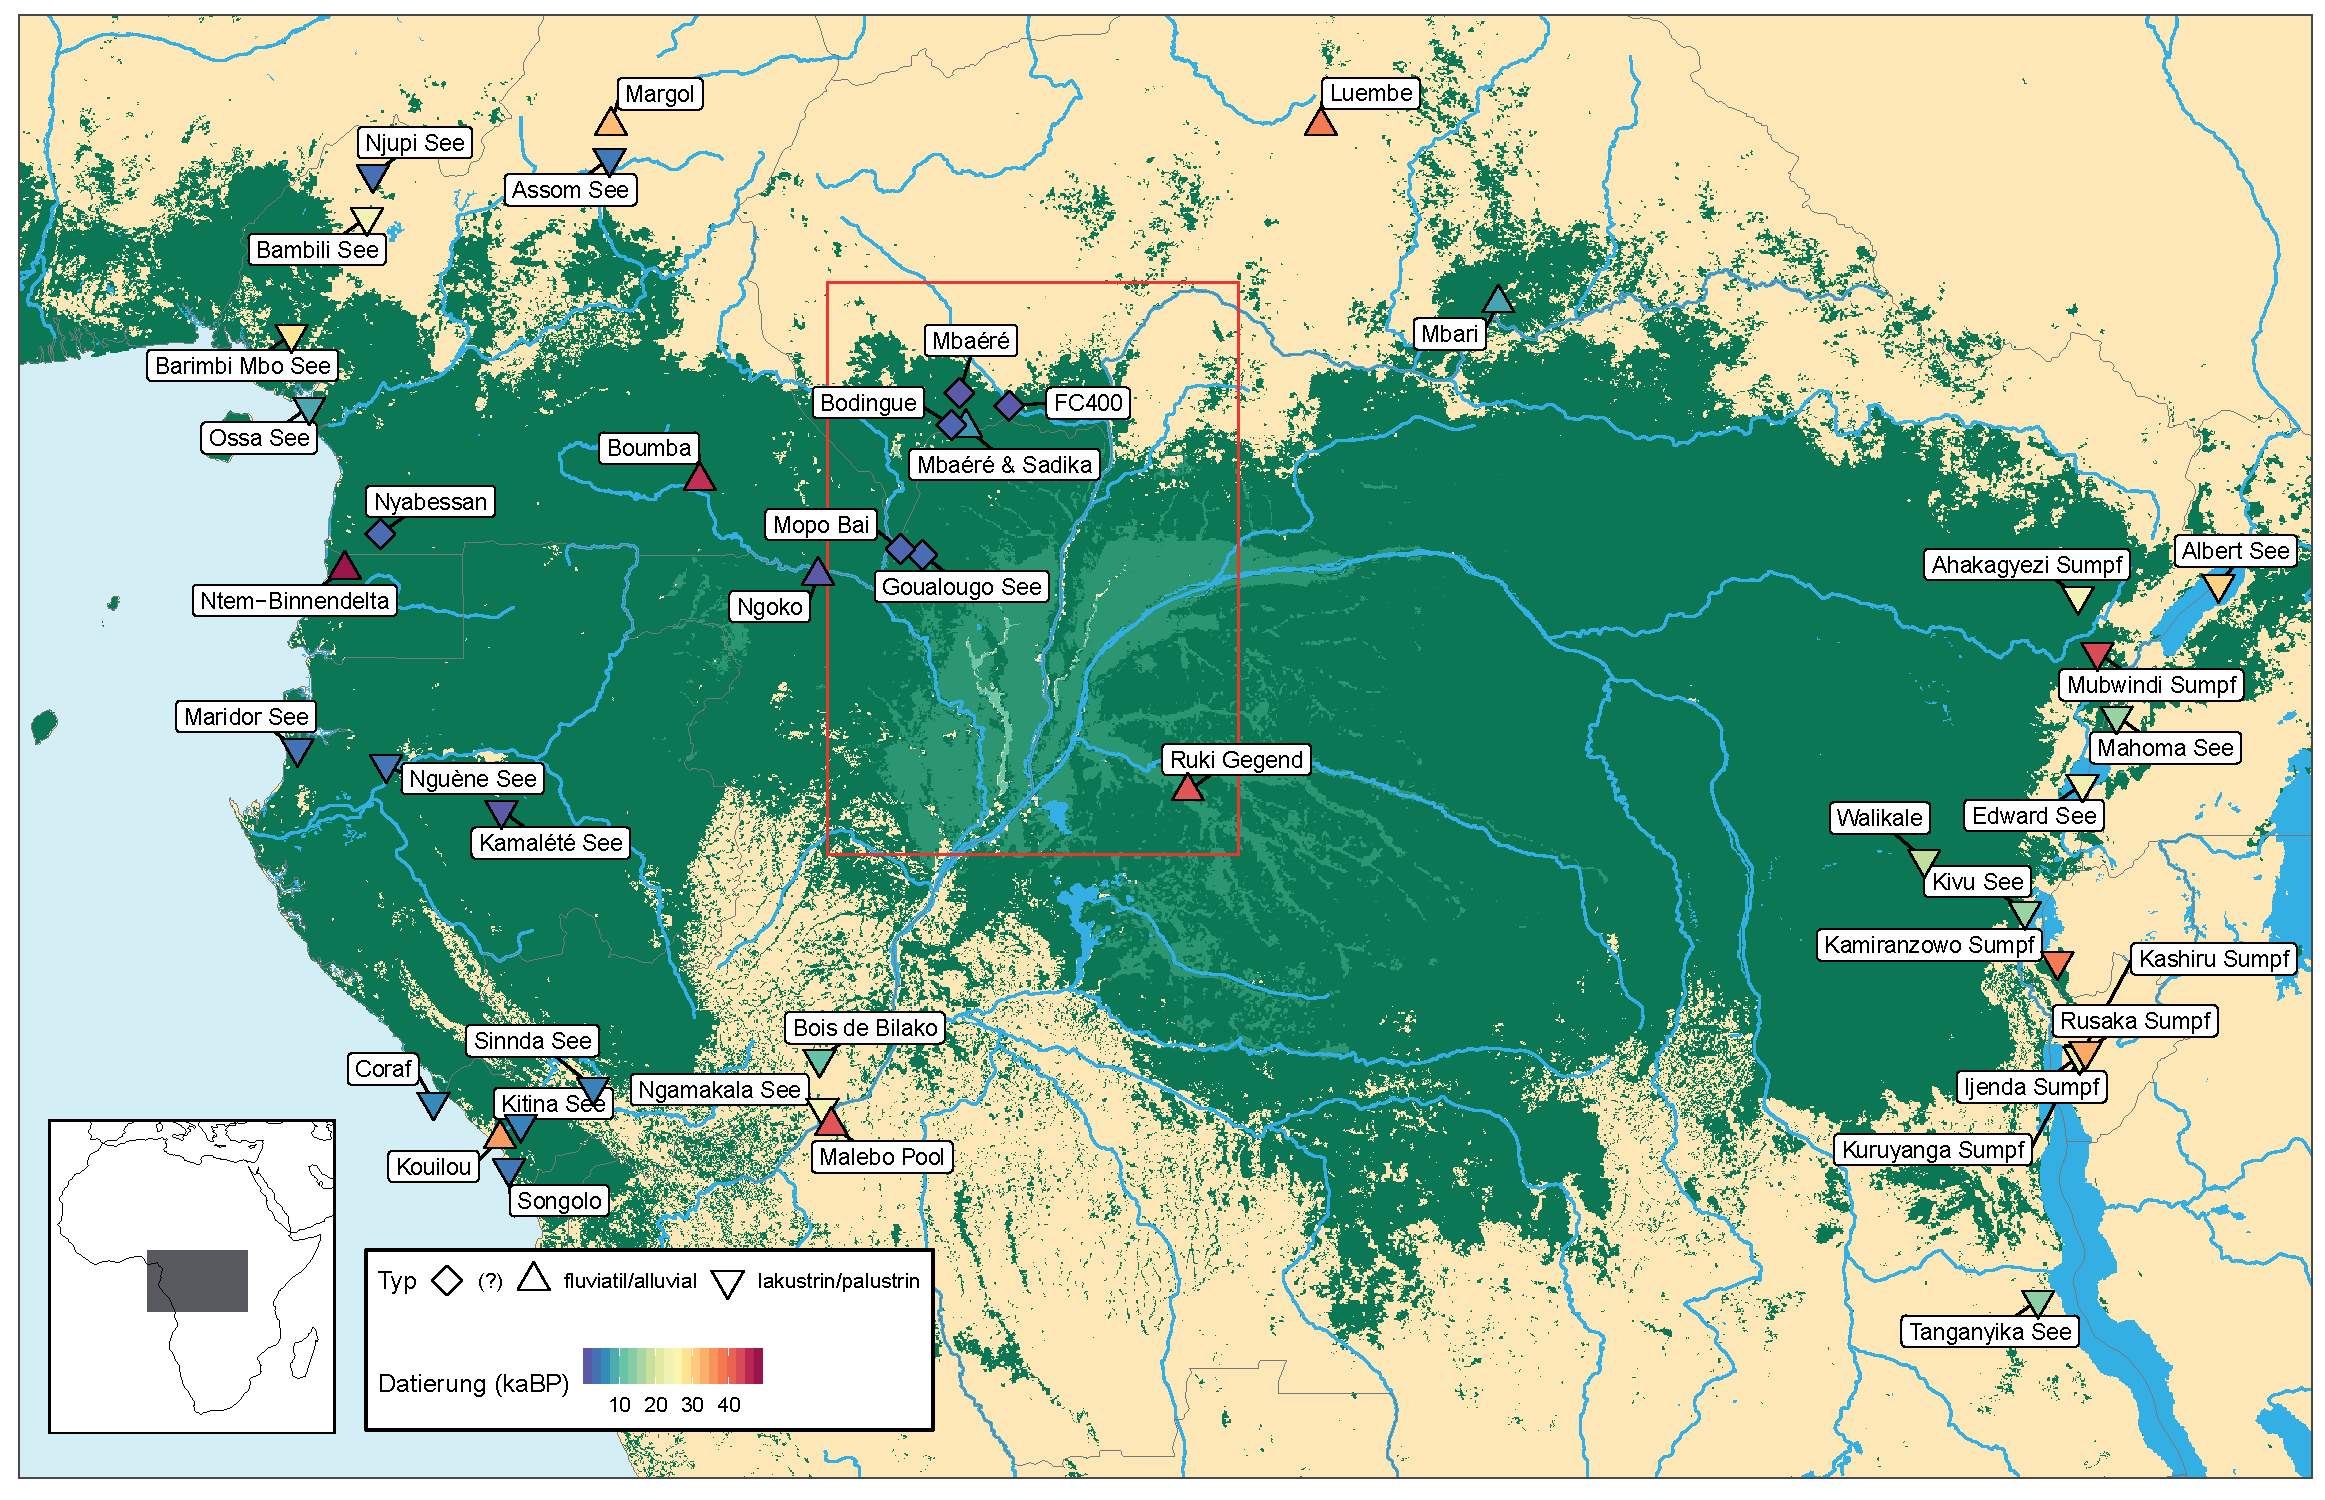
\includegraphics[width=\textwidth]{fig/Ch1_Fig2_PalaoUmwelt.pdf}
	\caption{Paläo-Umweltarchive und Vegetation: Kartierung der wichtigsten lakustrinen und palustrinen sowie fluviatilen und alluvialen Paläo-Umweltarchive sowie das maximale Alter der Ablagerungen \parencites[nach][]{Brncic.2007}{Brncic.2009}[43 Abb.~16, 46 Abb.~17]{Sangen.2009}{Kiahtipes.2011}{Kiahtipes.2016}. Rezente Verbreitung des immergrünen tropischen Regenwaldes (dunkelgrün) sowie Sumpfwald (hellgrün) nach \textcite{Mayaux.2003}. Das Arbeitsgebiet ist in rot hervorgehoben (siehe Abb.~\ref{fig:ArbeitsgebietKarte}).}
	\label{fig:PalaeoumweltArch_Karte}
\end{figure*}

Die Sichtweise, dass der tropische ombriophile Regenwald ein statisches Landschaftselement sei, konnte durch neuere Forschungen revidiert werden \parencite[83]{Runge.2001}. Es zeigte sich, dass der komplette Regenwald innerhalb von 40--100 Jahren durch einen komplexen Prozess kreislauforientierter Biomasseumsätze abgebaut und erneuert werden kann. Der immergrüne Regenwald des Inneren Kongobeckens bildet sich ab etwa 1600\,mm mittleren Jahresniederschlags aus (ebd. 83). Während der Waldbestand auf den Grundgebirgs-Latosolen im Randbereich homogen ist, zeigten sich im saisonal überfluteten Zentrum des Kongobeckens stärker heterogene Arten-Zusammensetzungen (ebd. 83\,f.). Die tropischen Wälder müssen folglich als \enquote{entwicklungsgeschichtlich und vom Standort abhängige, differenzierte Ökosysteme} (ebd. 92) betrachtet werden.

Beruhend auf der rezenten Variabilität des Baumartenbestandes wurde von \textcite{Maley.2001} die Ausdehnung des westlichen zentralafrikanischen Regenwaldes im ersten vorchristlichen Jahrtausend rekonstruiert. Diese zeigt ein zum heutigen Stand deutlich reduziertes und auf sogenannte \enquote{Refugien} begrenztes Verbreitungsbild. Die Nordgrenze der von \textsc{Maley} (ebd. 7 Abb.~4) postulierten Regenwaldverbreitung im Bereich des Laufs des \mbox{Ubangi} lag mutmaßlich deutlich südlich von Bangui (Fpl.~215) im Bereich zwischen Imese (Fpl.~201) und Dongo (Fpl.~202). Durch die ebenfalls postulierte Unterbrechung der Regenwaldverbreitung im Gebiet des \mbox{Sangha}, dem sogenannten \enquote{\mbox{Sangha}-Korridor}\footnote{Der auch \enquote{\mbox{Sangha}-Intervall} genannte Bereich beschreibt eine Zone zwischen 14--18$^\circ$~O, in der auffällige Pflanzengemeinschaften beobachtet werden können, die nicht zu den heutigen klimatischen Rahmenbedingungen der Region passen \parencite{Gond.2013}. Zu diesen Auffälligkeiten zählen die Anwesenheit der senegalesischen Dattelpalme (\textit{Phoenix reclinata}), die nirgends sonst im Regenwald beobachtet werden kann. Andererseits fehlen in dieser Region auch einige, für den äquatorialen Regenwald weiter westlich wie östlich charakteristische Pflanzen \parencite[356\,f.]{Bostoen.2015}. Entsprechende Beobachtungen ließen bereits \textcite{Letouzey.1968} eine potenzielle Verbindung zwischen dem nördlichen und südlichen Savannengürtel postulieren.\label{ftn:SanghaIntervall}} \parencites[siehe][]{Russell.2014}{Bostoen.2015} soll sich eine Grenze der Regenwaldverbreitung südlöstlich von Ouesso (Fpl.~265) ergeben haben.

Im engeren Arbeitsgebiet kamen in den letzten Jahren einige Paläo-Umweltarchive hinzu \parencites[siehe][]{Brncic.2007}{Brncic.2009}{Kiahtipes.2011}{Kiahtipes.2016}. Archive sind auch aus Kamerun, Gabun und dem Mündungsgebiet des Kongo bekannt \parencite[siehe][41--58; Abb.~\ref{fig:PalaeoumweltArch_Karte}]{Sangen.2009}. Während es im westlichen Zentralafrika\footnote{Gemeint sind hier die Staatsgebiete von Kamerun und Gabun sowie der Bereich der Kongomündung.} sowie im östlichen Zentral- und in Ostafrika -- vornehmlich in der Region der großen ostafrikanischen Seen -- eine Vielzahl von lakustrinen und palustrinen Paläo-Umweltarchiven gibt, liegen aus dem Kongobecken keine entsprechenden Archive vor (ebd. 54 Abb.~16). Mit Blick auf die fluvialen und alluvialen Paläoumweltarchive sieht die Situation insofern besser aus, als hier die Arbeiten von Johannes \textcites{Preu.1986}{Preu.1986b}{Preu.1990} im Bereich des Ruki genannt werden können. Weitere Untersuchungen fanden am Rand des Kongobeckens in einem Talabschnitt des Mbaéré im Südwesten der Zentralafrikanischen Republik statt \parencite{Neumer.2007}.

Die Rekonstruktion extralokaler Einflüsse auf die Ökologie aus punktuellen Ergebnissen und regionalen Vergleichen bildet eine der grundlegenden Schwierigkeiten für physiogeografische und umweltgeschichtliche Untersuchungen \parencite[42]{Sangen.2009}.\footnote{Die jüngste Phase der Erforschung der Landschaftsgeschichte Zentralafrikas wird von modernen Fernerkundungsverfahren bestimmt \parencite[6]{Runge.2001}. Die grundsätzlich schlechten Erhaltungsbedingungen für Pollen in den für gewöhnlich groben und stark oxidierten meso- bis cenozoischen Ablagerungen des Kongobeckens erschweren palynologische Studien. Als Folge verschob sich der Fokus paläoklimatologischer Untersuchungen in den Bereich geochemischer Analysen und der Untersuchung der sub-marinen Ablagerungen des Kongo-Schwemmkegels \parencite[312]{Giresse.2005b}. Die Turbidit-Ablagerungen im Kongo-Canyon sind ein direktes Resultat der Suspensionsfracht des Kongo und repräsentieren dessen Schwankungen im Zusammenhang mit Faktoren wie Meeresspiegelschwankungen, Tektonik und Klimaveränderungen \parencite[2176]{Savoye.2009}.} Für den Gegenstand dieser Arbeit sind vornehmlich die Einflüsse des Ökosystems und dessen Veränderungen auf die menschliche Besiedlung des Kongobeckens von Bedeutung. Aus dem tropischen Afrika liegen insgesamt nur sehr wenige komplette, vom Ende der letzten Eiszeit bis in die Gegenwart reichende Pollenprofile vor \parencite[2682]{Lezine.2013}, so zum Beispiel das Profil aus dem Sacred Lake in Kenia \parencite[65--73; Beilage Fig.~15]{Coetzee.1967} sowie jenes aus dem Barombi-Mbo-See in Kamerun \parencite{Maley.1991}. Für das Pleistozän im Inneren Kongobecken liegen lediglich vorläufige Untersuchungsergebnisse aus Analysen durch Emile Roche vor, wonach Pollen aus der Ruki- und Momboyo-Region auf eine offene Savannen-Landschaft sowie nahe Marsch-Areale und Galleriewälder hinweisen würden \parencite[181]{Fiedler.1985}.\footnote{Für die Untersuchung wurden organisch reiche Sedimentschichten aus Imbonga am Momboyo \parencite[siehe][542\,f. Karte~1 Fpl.~43]{Wotzka.1995} sowie Bokuma-Isoko am Ruki (Fpl.~18) analysiert, welche zwischen 25\,000--15\,000 bp datieren \parencite[182]{Fiedler.1985}. Eine direkte Publikation dieser Daten liegt nicht vor.}

Eines der aussagekräftigsten Paläo-Umweltarchive, durch das eine Rekonstruktion der Klimaentwicklung der Großregion möglich wird, stammt aus dem knapp 2\,km großen, nahezu kreisrunden und 110\,m tiefen Vulkansee Barombi Mbo in Westkamerun \parencite[159--161]{Maley.1998b}.\footnote{Der in der Seemitte genommene, 23,5\,m lange Sedimentkern BM-6 enthielt Schichten, die zirka 27\,500 Jahre zurückreichen, wobei die untersten 1,5\,m des Kerns eine, vermutlich durch vulkanische Aktivität verursachte, gestörte Lagerung aufwiesen \parencite[6 Abb. 1]{Maley.2001}. Auch aufgrund der allgemeinen Schwierigkeiten einer \textsuperscript{14}C-Datierung in diesen Zeiträumen werden die ältesten ansprechbaren Schichten auf vor 24\,000 Jahren datiert. Die Daten zeigen im für diese Arbeit wichtigen 1.~Jt. v.~Chr. einen Rückgang der Regenwald-Flora beziehungsweise Baumpollen zugunsten von Savannen-Taxa  \parencites[6 Abb. 1]{Maley.2001}[56--58]{Maley.2003}.} Mit Blick auf die Erkenntnisse aus dem Barombi Mbo-Kern wurden von \textcite[357--360]{Schwartz.1992} erstmals Überlegungen zu den Zusammenhängen zwischen der Aufsiedlung des zentralafrikanischen Regenwaldes durch keramikproduzierende und sesshaftlebende Gruppen in der zweiten Hälfte des 1.~Jt. v.~Chr., der Ausbreitung der Eisenmetallurgie in den letzten Jahrhunderten vor der Zeitenwende sowie der heute unter den Begriffen \textit{First Millennium BC Crisis} \parencite[63]{Sangen.2009} beziehungsweise \enquote{Krise des Regenwaldes} \parencite{Neumann.2014} bekannten klimatischen sowie damit einhergehenden ökologischen Veränderung des Regenwaldes nach etwa 1000 v.~Chr. angestellt.

Die Veränderung der Regenwald-Vegetation im 1.~Jt. v.~Chr. lässt sich auch im Pollenprofil aus dem Nyabessan-Sumpf im Ntem-Binnendelta in Südkamerun nachvollziehen \parencite[316]{Ngomanda.2009}. So zeichnet sich gegen 500 v.~Chr. in den Daten ein deutlicher Wandel der Regenwaldflora ab. Das zirka 1,8\,m mächtige und vom 13./11. bis in das 5./3.~Jh. v.~Chr. datierende Profil zeigt für die zweite Hälfte des 1.~Jt. v.~Chr. einen Rückgang des Sekundärwaldes zugunsten eines Anstiegs von Primärwald-Taxa \parencite[ebd. 311 Abb.~3; ][58 Abb.~5]{Neumann.2012}.

Daten für die holozäne Klimageschichte des Arbeitsgebietes liegen aus dem südlichen Teil des \enquote{Nouabalé-Ndoki National Park}, in der nördlichen Republik Kongo vor \parencite{Brncic.2007}.\footnote{Ein etwa 68\,cm langer Sedimentkern aus dem Goualougo-See deckt die letzten 3300~Jahre ab (\textsc{Brncic, Willis} u.~a. 2007: 236--237 Abb.~59). Die Untersuchung ergab, dass sich überregionale klimatische Vorgänge kaum niedergeschlagen haben, da feuchte semi-immergrüne Waldtaxa durch die gesamte, durch den Kern abgedeckte Zeit hindurch konstant vorkamen (ebd. 240). Anzeichen für eine Savannen-Ausbreitung konnten nicht beobachtet werden. In den vergangenen 1000 Jahren mehren sich Anzeichen für anthropogene Feuer. Verschiedene Pioniertaxa wie \textit{E. guineensis}, \textit{Tetrorchidium} sp. und \textit{Erythrophleum} sp. zeigen trockenere Perioden an (ebd.). Das Vorkommen dieser Taxa ist fast ausschließlich auf das 1.~Jt. v.~Chr. beschränkt (ebd. 236 Fig.~5).} Der anthropogene Einfluss auf die Vegetation der Region innerhalb der letzten 3000~Jahre ist demnach größer als jener der auf klimatische Veränderungen zurückgeht. Ein zweiter Sedimentkern stammt aus Mopo Bai, einer saisonal überfluteten, sumpfigen Niederung etwa 28\,km westnordwestlich des Goualougo-Sees \parencite[80]{Brncic.2009}. Der 1\,m lange Kern deckt die letzten 2500~Jahre ab und die Pollensequenz zeigt deutliche Einflüsse klimatischer und anthropogener Faktoren auf die Ökologie (ebd. 86). Die Holzkohlekonzentration nimmt ab dem 11.~Jh. n.~Chr. in Form mehrerer, ansteigender Spitzenwerte zu (ebd. 85 Abb.~5) und der Anteil von \textit{Elaeïs guineensis} -- einer Pioniertaxa -- ist um die Zeitenwende am größten und nimmt ab dann stetig ab (ebd. 83 Abb.~4).

Aus dem Ngotto-Waldschutzgebiet im äußersten Südwesten der Zentralafrikanischen Republik ist die Untersuchung von zwei Pollenkernen bekannt \parencite{Kiahtipes.2011}. Ein Sedimentkern wurde 2007 aus der Flussmarsch des Bodingue gezogen.\footnote{Der insgesamt 72\,cm lange Kern wurde in Abständen von 10\,cm beprobt. Drei aus dem oberen, mittleren und unteren Bereich des Kerns genommene \textsuperscript{14}C-Proben zeigen an, dass er eine Zeitspanne vom 5.~Jh. v.~Chr. bis zum 13.~Jh. n.~Chr. abdeckt (\textsc{Kiahtipes} u.~a. 2011: 4 Tab.~1; 5 Fig.~2).} Ein zweiter Kern stammt aus der Uferzone der Flussmarsch des Mbaéré.\footnote{Der 2,5\,m lange Kern wurde in Intervallen von 5\,cm beprobt. In die Analyse ging nur jede zweite Probe ein. Der Kern deckt eine Zeitspanne vom 7./8.~Jh. n.~Chr. bis in die Gegenwart ab (\textsc{Kiahtipes} u.~a. 2011: 11 Fig.~6).} Kombiniert bietet sich durch beide Kerne ein Einblick in die regionale Entwicklung für die letzten etwa 2500 Jahre (ebd. 4 Tab.~1, 5 Fig.~2). Nahe des Zusammenflusses der Flüsse Loame und Lobaye wurde in einer Region mit Feuchtsavannen-Vegetation ein 2\,m langer Sedimentkern erbohrt \parencite[5]{Lupo.2015}. Radiokohlenstoffdatierungen zeigten, dass der Kern Paläo-Umweltdaten der letzten 500 Jahre abdeckt (ebd. 13 Abb.~6). In der Auswertung zeigte sich ein Wechsel von einer dichten Regenwaldvegetation zu einer offeneren, savannenartigeren Vegetation im späten 17. oder frühen 18.~Jh.
\end{multicols}